%# -*- coding: utf-8 -*-
%!TEX encoding = UTF-8 Unicode
%%%%%%%%%%%%%%%%%%%%%%%%%%%%%%%%%%%%%%%%%%%%%%%%%%%%%%%%%%%%%%%%%%%%%%%%%%%%%%%%%%
%论文模板                                                                        %
%此为中文XeLatex-article                                                         %
%                             !编译方式是:XeLaTeX  !                          %
%%%%%%%%%%%%%%%%%%%%%%%%%%%%%%%%%%%%%%%%%%%%%%%%%%%%%%%%%%%%%%%%%%%%%%%%%%%%%%%%%%
\documentclass[12pt]{article}
\usepackage[slantfont,boldfont]{xeCJK}% 允许斜体和粗体
\setCJKmainfont{FangSong}             % 设置缺省中文字体
\setmainfont{Times New Roman}         % 设置Times New Roman为默认的英文字体
\setlength{\parindent}{2.5em}         % 中文缩进两个汉字位

\usepackage{CJK}
\usepackage{titlesec}%章节标题格式设置
\usepackage{titletoc}%目录格式设置
\usepackage{amsmath}%公式环境数学命令
\usepackage{array}%数组和表格制作
\usepackage[a4paper,top=2.5cm,bottom=2.5cm,left=3cm,right=2cm]{geometry}% 版面尺寸设置
\usepackage{multirow}
\usepackage{enumerate}
\usepackage{verbatim,listings}
\usepackage{color,xcolor}
%\usepackage{graphicx}
\usepackage{slashbox}
\usepackage{fancybox}
\usepackage{fancyhdr}
\usepackage{float}    % for fig.pos='H'
\usepackage{rotfloat} % for sidewaysfigure
\usepackage{subfig}   % for subfigure
\usepackage{booktabs}

%%%%%%%%%%%%%%%%%%%%%%%%%%%%%%%%%%%%%%%%%%%%%%%%%%%%%%%%%%%%%%%%%%%%%%%%%%%%%%%%%%%%%%%%%%%%%%%%%%%%%
%自定义命令:
\makeatletter
%字号设置
\newcommand{\chuhao}{\fontsize{42pt}{\baselineskip}\selectfont}% 初号
\newcommand{\xiaochuhao}{\fontsize{36pt}{\baselineskip}\selectfont}% 小初号
\newcommand{\yihao}{\fontsize{28pt}{\baselineskip}\selectfont}% 一号
\newcommand{\erhao}{\fontsize{21pt}{\baselineskip}\selectfont}% 二号
\newcommand{\xiaoerhao}{\fontsize{18pt}{\baselineskip}\selectfont}% 小二号
\newcommand{\sanhao}{\fontsize{15.75pt}{\baselineskip}\selectfont}% 三号
\newcommand{\xiaosanhao}{\fontsize{15pt}{\baselineskip}\selectfont}% 小三号
\newcommand{\sihao}{\fontsize{14pt}{\baselineskip}\selectfont}% 四号
\newcommand{\xiaosihao}{\fontsize{12pt}{\baselineskip}\selectfont}% 小四号
\newcommand{\wuhao}{\fontsize{10.5pt}{\baselineskip}\selectfont}% 五号
\newcommand{\xiaowuhao}{\fontsize{9pt}{\baselineskip}\selectfont}% 小五号
\newcommand{\liuhao}{\fontsize{7.875pt}{\baselineskip}\selectfont}% 六号
\newcommand{\qihao}{\fontsize{5.25pt}{\baselineskip}\selectfont}% 七号

%行间距设置
\renewcommand\baselinestretch{1.25}%1.25倍行距

%页眉页脚设置1
\fancypagestyle{plain}
{
\fancyhead{}
\fancyhead[C]{\wuhao{数理与土木工程学院大数据系实验报告}}
\fancyfoot{}
\fancyfoot[C]{\thepage}
}
%页眉页脚设置2
\pagestyle{fancy}
{
 \fancyhead{}
 \fancyhead[C]{\wuhao{数理与土木工程学院大数据系实验报告}}
 \fancyfoot{}
}

%重新定义
\renewcommand\refname{参考文献}
\renewcommand\figurename{图}
\renewcommand\tablename{表}

%表格设置
\newsavebox{\tablebox}


\makeatother
%%%%%%%%%%%%%%%%%%%%%%%%%%%%%%%%%%%%%%%%%%%%%%%%%%%%%%%%%%%%%%%%%%%%%%%%%%%%%%%%%%%%%%%%%%%%%%%%%%%%%


\begin{document}

\lstset{numbers=left,
numberstyle= \tiny,
keywordstyle= \color{ blue!70},commentstyle=\color{red!50!green!50!blue!50},
frame=shadowbox,
rulesepcolor= \color{ red!20!green!20!blue!20}
}
\lstset{
  breaklines,%自动换行
  columns=flexible,%不随便添加空格,只在已经有空格的地方添加空格,
%如果想要添加空格使用fixed作为参数(这是默认的),如果坚决不添加空格使用fullflexible作为参数.
}

%%%%%%%%%%%%%%%%%%%%%%%%%%%%%%%%%%%%%%%%%%%%%%%%%%%%%%%%%%%%%%%%%%%%%%%%%%%%%%%%%%%%%%%%%%%%%%%%%%%%%%

%%%%%%%%%%%%%%%%%%封面%%%%%%%%%%%%%%%%%%%%%%%%%%%%%%%%%%%%%%%%%%%%%%%%%%%%%%%%%%%%%%%%%%%%%%%%%%%%%%%%%
\thispagestyle{empty}

\begin{center}

\includegraphics[height=0.15\textwidth]{figures/logo.jpg}

\vspace{4cm}

{\yihao\bf{Linux中基于mysql,hive,sqoop安装及操作}}
\end{center}

\vspace{4cm}

{\xiaosanhao\bf
\begin{center}
\makebox[3cm][l]{学~~~~~~~~~院:}\underbar{\makebox[11cm][c]{数理与土木工程学院}}
\end{center}
\begin{center}
\makebox[3cm][l]{课~~~~~~~~~程:}\underbar{\makebox[11cm][c]{大数据工具箱1}}
\end{center}
\begin{center}
\makebox[3cm][l]{班~~~~~~~~~级:}\underbar{\makebox[11cm][c]{数据科学与大数据技术1班}}
\end{center}
\begin{center}
\makebox[3cm][l]{姓~~~~~~~~~名:}\underbar{\makebox[4cm][c]{覃诗杰}}\makebox[3cm][l]{学~~~~~~~~~号:}\underbar{\makebox[4cm][c]{201205102261}}
\end{center}
}


\vspace{4cm}


\begin{center}\wuhao\bf
{
\makebox[5cm][c]{中国~$\cdot$~珠海}

\renewcommand{\today}{\number\year 年 \number\month 月 \number\day 日}
\today\\
%\makebox[5cm][c]{二〇二〇年六月}
}

\end{center}
%%%%%%%%%%%%%%%%%%%目录%%%%%%%%%%%%%%%%%%%%%%%%%%%%%%%%%%%%%%%%%%%%%%%%%%%%%%%%%%%%%%%%%%%%%%%%%%%%%
\newpage

\thispagestyle{fancy}

\vspace*{1mm}%垂直距离


\renewcommand\contentsname{\xiaosanhao\textbf{目~~~录}}


\tableofcontents
%%%%%%%%%%%%%%%%%%%正文:第1部分%%%%%%%%%%%%%%%%%%%%%%%%%%%%%%%%%%%%%%%%%%%%%%%%%%%%%%%%%%%%%%%%%%%%%
\newpage%新的一页

\pagestyle{plain}
\pagenumbering{arabic}


\section{实验背景}
\noindent\qquad MySQL是一个关系数据库管理系统,由瑞典MySQL AB公司开发,目前属于Qracle旗下的产品。MySQL是流行的关系数据库管理系统,在Web应用方面,MySQL是最好的关系数据库管理系统应用软件之一。

\noindent\qquad HIVE是一种底层封装了Hadoop 的数据仓库处理工具,使用类SQL 的hiveSQL 语言实现数据查询,所有hive 的数据都存储在Hadoop 兼容的文件系统(例如,Amazon S3、HDFS)中。. hive 在加载数据过程中不会对数据进行任何的修改,只是将数据移动到HDFS 中hive 设定的目录下,因此,hive 不支持对数据的改写和添加,所有的数据都是在加载的时候确定的。

\noindent\qquad Sqoop (发音:skup)是一款开源的工具,主要用于在Hadoop (Hive)与传统的数据库 (mysql、postgresql...)间进行数据的传递,可以将一个 关系型数据库 (例如 : MySQL,Oracle,Postgres 等) 中的数据导进到Hadoop的HDFS中,也可以将HDFS的数据导进到关系型数据库中。

\noindent\qquad Sqoop的安装与Mysql的数据导入到hdfs框架中 Sqoop (发音:skup)是一款开源的工具,主要用于在Hadoop (Hive)与传统的数据库 (mysql)间进行数据的传递
\section{实验目的}
我们可以使用sqoop工具,将业务数据库mysql或者oracle中的数据落地到hive表中,以方便后续的大数据统计分析。

\section{实验环境}
VirtualBox 6.1.14, Ubuntu 16.04,mysql-connector-java-5.1.40,apache-hive-1.2.1-bin,sqoop-1.4.7

\noindent\qquad 在结尾参考文献中,有本文用到的所有包
\section{实验任务及完成过程}
\noindent\qquad 任务一:安装下载mysql,所以操作mysql是为基础,然后再进行简单的操作介绍

\noindent\qquad 任务二:安装hive,与mysql互通,hive与本地文件互传,hive与分布式数据互通,再做一个实例

\noindent\qquad 任务三:基于任务一和任务二,配置环境路径,安装sqoop,进行数据传输操作

\section{MYSQL}
\subsection{安装MySQL以及问题处理}

(1)更新软件源,安装mysql
\begin{lstlisting}[language={[ANSI]C}]
sudo apt-get update
sudo apt-get install mysql-server
\end{lstlisting}


(2)启动时可能遇到密码错误原因,直接跳过验证密码,在sudo vim /etc/mysql/my.cnf中编辑加入两行代码
\begin{lstlisting}[language={[ANSI]C}]
[mysqld]
skip-grant-tables
\end{lstlisting}


\begin{figure}[ht]
\centering
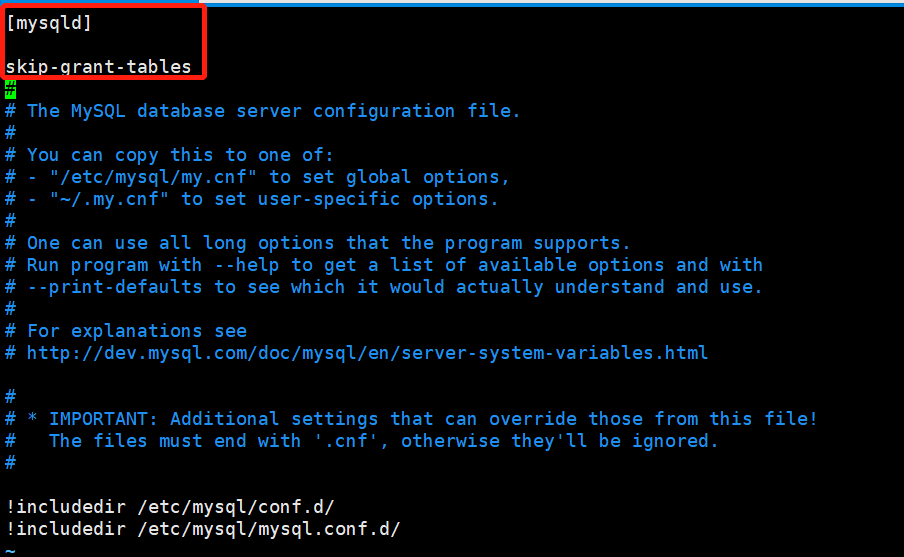
\includegraphics[scale=0.7]{figures/1.png}
\caption{加入权限}\label{fig:label2}
\end{figure}

\begin{figure}[ht]
\centering
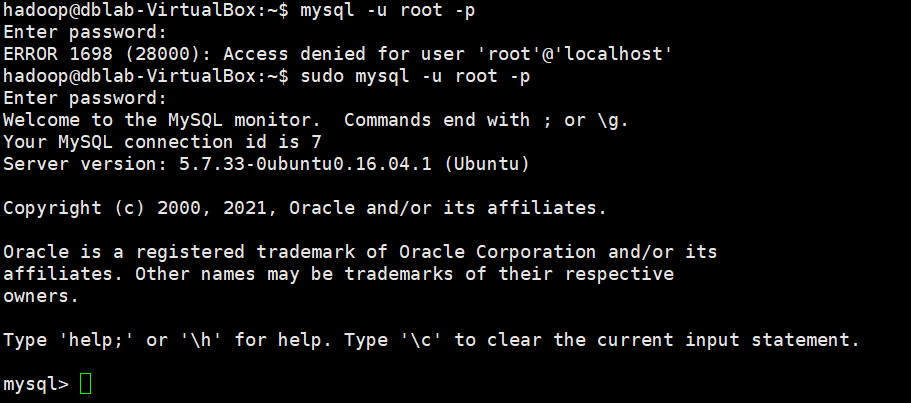
\includegraphics[scale=0.8]{figures/2.png}
\caption{进入mysql跳过密码}\label{fig:label2}
\end{figure}

\newpage

(3) 权限不够的报错信息,如图

\begin{figure}[ht]
\centering
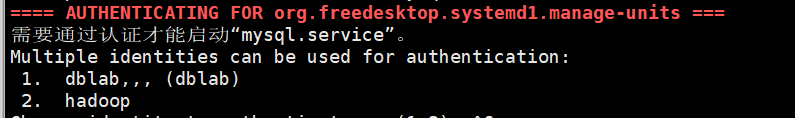
\includegraphics[scale=1.1]{figures/3.png}
\caption{权限不够}\label{fig:label2}
\end{figure}

(3) 增加权限
\begin{lstlisting}[language={[ANSI]C}]
sudo service mysql start
\end{lstlisting}



\subsection{MySQL的启动}

(1)开启,关闭mysql
\begin{lstlisting}[language={[ANSI]C}]
service mysql stop
service mysql start
\end{lstlisting}
(2)查看是否开启进程
\begin{lstlisting}[language={[ANSI]C}]
ps  ajx|grep xxx比如mysql,redis
\end{lstlisting}

\begin{figure}[ht]
\centering
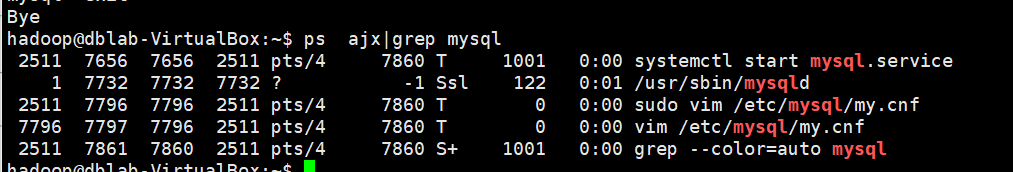
\includegraphics[scale=0.9]{figures/5.png}
\caption{查看mysql进程}\label{fig:label2}
\end{figure}

\subsection{MySQL创建数据库和数据表}
(1)创建数据库,删除数据库
\begin{lstlisting}[language={[ANSI]C}]
CREATE DATABASEexample;
DROP DATABASEexample;
\end{lstlisting}

(2)创建表,例:
\begin{lstlisting}[language={[ANSI]C}]
CREATE TABLEstudent (-> id int,-> name varchar(20)->);
\end{lstlisting}

(3)查看数据库
\begin{lstlisting}[language={[ANSI]C}]
show databas
\end{lstlisting}


\begin{figure}[ht]
\centering
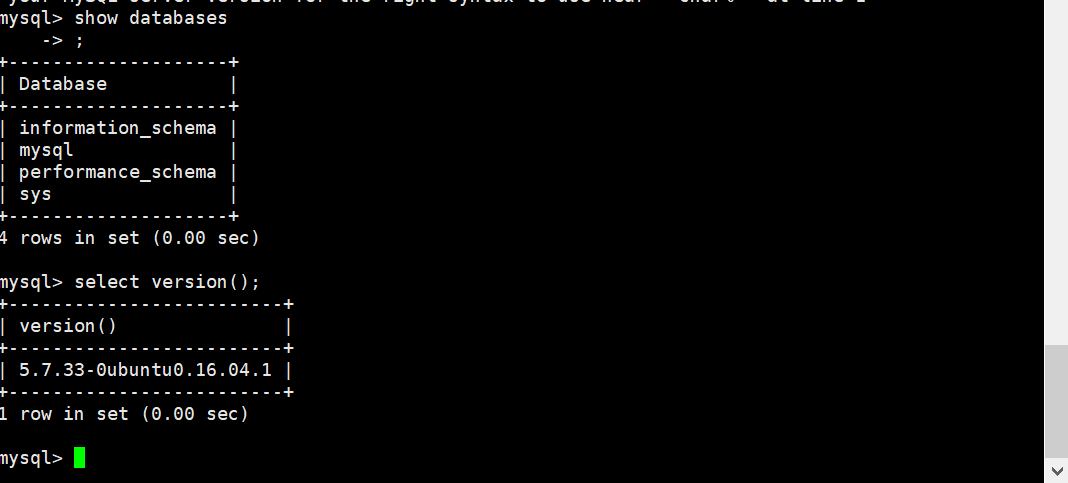
\includegraphics[scale=0.8]{figures/4.png}
\caption{查看数据库}\label{fig:label2}
\end{figure}


\section{HIVE}

\subsection{安装过程和配置环境变量}

(1)安装和配置环境变量
\begin{lstlisting}[language={[ANSI]C}]
sudo tar -zxvf ./apache-hive-1.2.1-bin.tar.gz -C /usr/local
cd /usr/local/
sudo mv apache-hive-1.2.1-bin hive
sudo chown -R hadoop:hadoop hive
\end{lstlisting}

\begin{lstlisting}[language={[ANSI]C}]
vim ~/.bashrc
export HIVE_HOME=/usr/local/hive
export PATH=$PATH:$HIVE_HOME/bin
export HIVE_HOME=/usr/local/hive
export PATH=$PATH:$HIVE_HOME/bin
\end{lstlisting}

如图:

\begin{figure}[ht]
\centering
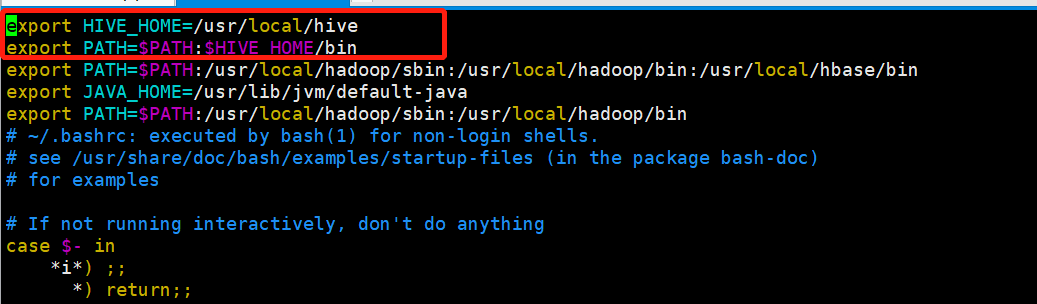
\includegraphics[scale=0.8]{figures/7.png}
\caption{配置}\label{fig:label2}
\end{figure}


\newpage
(2) 配置文件

\begin{lstlisting}[language={[ANSI]C}]
cd /usr/local/hive/conf
sudo mv hive-default.xml.template hive-default.xml
vim hive-site.xml
\end{lstlisting}

\begin{figure}[ht]
\centering
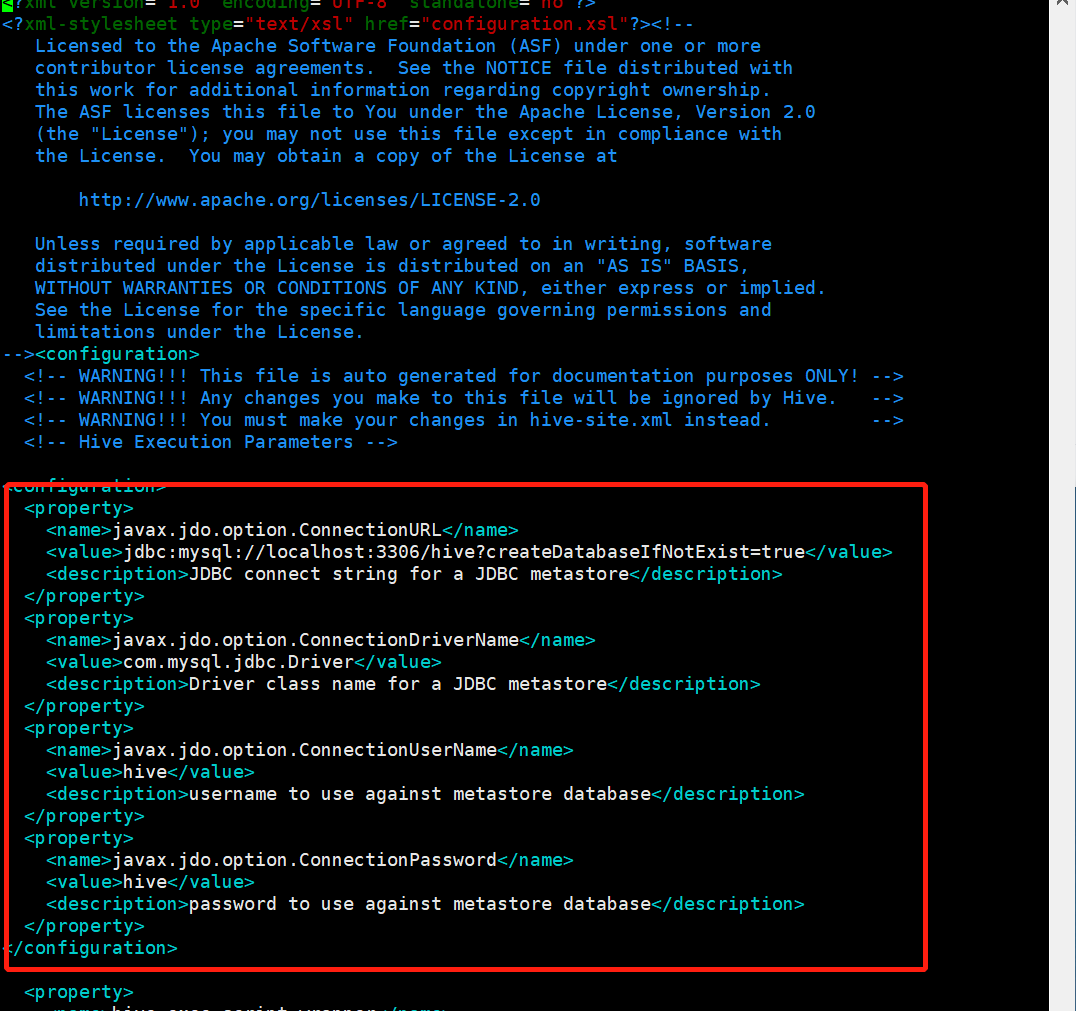
\includegraphics[scale=0.7]{figures/8.png}
\caption{增加一些配置}\label{fig:label2}
\end{figure}

(3) hive需要配置MySQL JDBC
\begin{lstlisting}[language={[ANSI]C}]
cd ~
tar -zxvf mysql-connector-java-5.1.40.tar.gz
cp mysql-connector-java-5.1.40/mysql-connector-java-5.1.40-bin.jar  /usr/local/hive/lib
\end{lstlisting}

(4)root密码为空的时候配置文件中下面这句
\begin{lstlisting}[language={[ANSI]C}]
skip-grant-tables
\end{lstlisting}

\newpage
(5) 配置hive连接mysql,mysql给权限给hive
\begin{lstlisting}[language={[ANSI]C}]
reate database hive;
#需要先输入下面这句话,才能正常运行
flush privileges;
grant all on *.* to hive@localhost identified by 'hive';
\end{lstlisting}

\subsection{基础操作}

(1)开启进程
\begin{lstlisting}[language={[ANSI]C}]
cd /usr/local/hadoop
./sbin/start-dfs.sh
\end{lstlisting}
(2)进入hive打开hive
\begin{lstlisting}[language={[ANSI]C}]
cd /usr/local/hive
./bin/hive
\end{lstlisting}

\begin{figure}[ht]
\centering
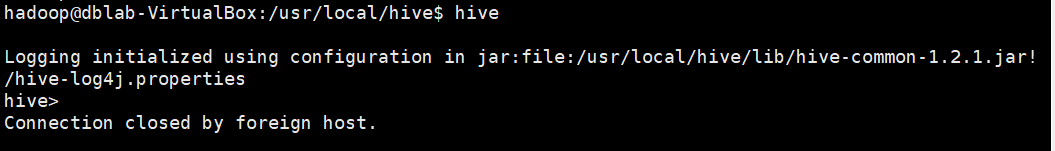
\includegraphics[scale=0.8]{figures/9.png}
\caption{成功}\label{fig:label2}
\end{figure}

(3)创建数据库
\begin{lstlisting}[language={[ANSI]C}]
create database hive;
create database if not exists hive;
\end{lstlisting}

\begin{figure}[ht]
\centering
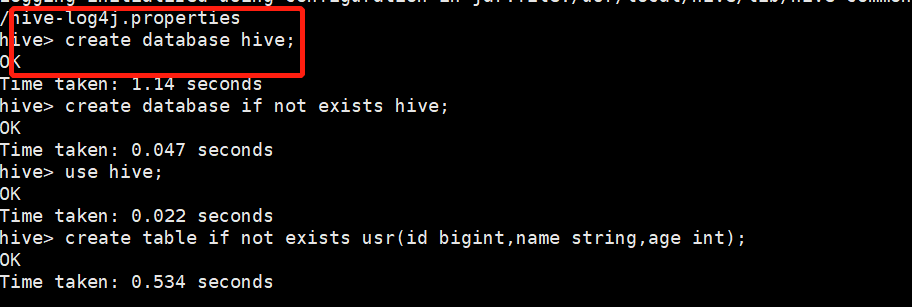
\includegraphics[scale=0.9]{figures/10.png}
\caption{创建数据库}\label{fig:label2}
\end{figure}

\newpage
(3)进入hive数据库,创建数据表,但是会出现一点点问题
\begin{lstlisting}[language={[ANSI]C}]
use hive;
create table if not exists usr(id bigint,name string,age int);
create table if not exists hive.usr(id bigint,name string,age int)location ‘/usr/local/hive/warehouse/hive/usr’;
\end{lstlisting}

\begin{figure}[ht]
\centering
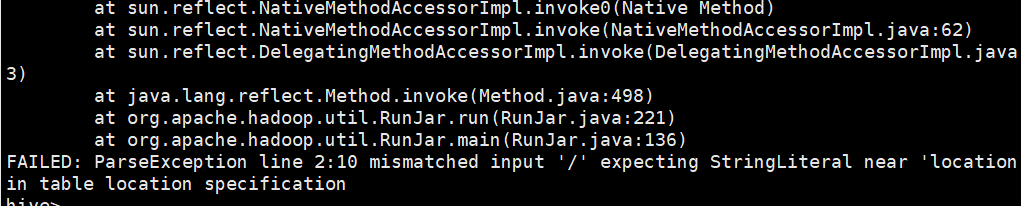
\includegraphics[scale=0.9]{figures/11.png}
\caption{报错}\label{fig:label2}
\end{figure}

(4)解决方法
\begin{lstlisting}[language={[ANSI]C}]
#修改字符
create table mypercent(id bigint,name string,age int)
row format delimited fields terminated by ',';
\end{lstlisting}

(5)删除数据库,数据表
\begin{lstlisting}[language={[ANSI]C}]
#删除数据库
drop database hive;
\end{lstlisting}

(6)无论有没有这个数据库都不会报错的删除
\begin{lstlisting}[language={[ANSI]C}]
drop database if exists hive;
\end{lstlisting}
(7)加上cascade关键字,可以删除当前数据库和数据表

\begin{lstlisting}[language={[ANSI]C}]
drop database if exists hive cascade;
\end{lstlisting}

(8)删除表
\begin{lstlisting}[language={[ANSI]C}]
drop table if exists usr;
\end{lstlisting}

(9)删除视图
\begin{lstlisting}[language={[ANSI]C}]
drop view if exists little_usr;
\end{lstlisting}

(10)查看表,查看数据库
\begin{lstlisting}[language={[ANSI]C}]
show databases;
use hive;
show tables;
\end{lstlisting}

\begin{figure}[ht]
\centering
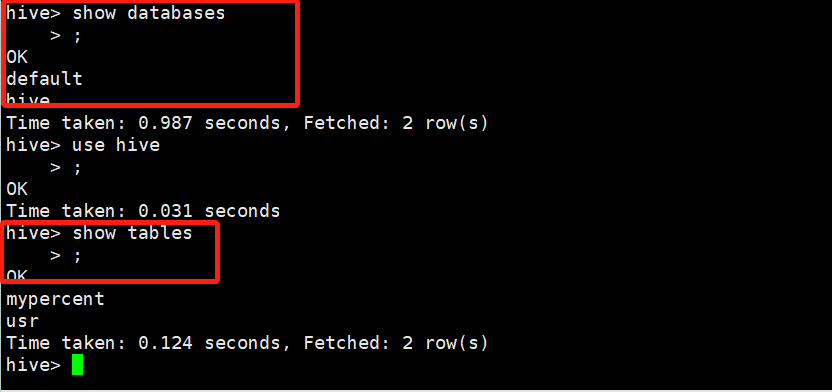
\includegraphics[scale=1.0]{figures/13.png}
\caption{结果}\label{fig:label2}
\end{figure}

(11)查看基本信息
\begin{lstlisting}[language={[ANSI]C}]
escribe hive.usr;
describe hive.little_usr;
#查看usr中的id
describe extended hive.usr.id;
\end{lstlisting}

\subsection{装载操作}

(1)把xxx数据文件装置到xxx表中并且覆盖原有文件

\begin{lstlisting}[language={[ANSI]C}]
load data local inpath ‘数据路径’ overwrite into table xxx;
\end{lstlisting}

(2)把xxx数据文件装置到xxx表中并且不覆盖原有文件
\begin{lstlisting}[language={[ANSI]C}]
load data local inpath ‘数据路径’ into table xxx;
#也就是覆盖用overwrite,不覆盖用into
\end{lstlisting}

(2)把在hdfs中的xxx数据文件装置到xxx表中并且覆盖原有文件

\begin{lstlisting}[language={[ANSI]C}]
load data inpath ‘hdfs://master_server/数据路径’ overwrite into table xxx;
\end{lstlisting}

\subsection{hive实例}

(1)在本地创建数据

\begin{lstlisting}[language={[ANSI]C}]
cd /usr/local/hadoop
vim employees.txt
#存入数据
\end{lstlisting}

\begin{table}[!ht]

    \centering
    \begin{tabular}{|l|l|l|l|l|}
    \hline
        1201 & Gopal & 45000 & Technical manager  & \\ \hline
        1202 & Manisha & 45000 & Proof reader  &  \\ \hline
        1203 & Masthanvali & 40000 & Technical writer  & \\ \hline
        1204 & Krian & 40000 & Hr Admin  &  \\ \hline
        1205 & Kranthi & 30000 & Op Admin & \\ \hline
        \bottomrule
    \end{tabular}
\end{table}

\begin{figure}[ht]
\centering
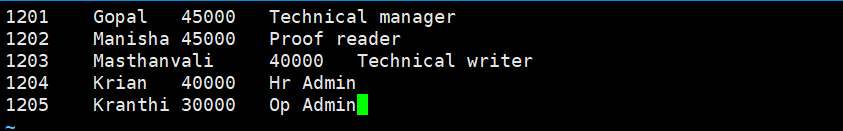
\includegraphics[scale=1.0]{figures/16.png}
\caption{数据准备}\label{fig:label2}
\end{figure}

(1)本地数据传入hive

\begin{lstlisting}[language={[ANSI]C}]
cd /usr/local/hadoop
vim employees.txt
#存入数据
load data local inpath '/usr/local/hadoop/employees.txt' into table employee;
select * from employee
\end{lstlisting}

\begin{figure}[ht]
\centering
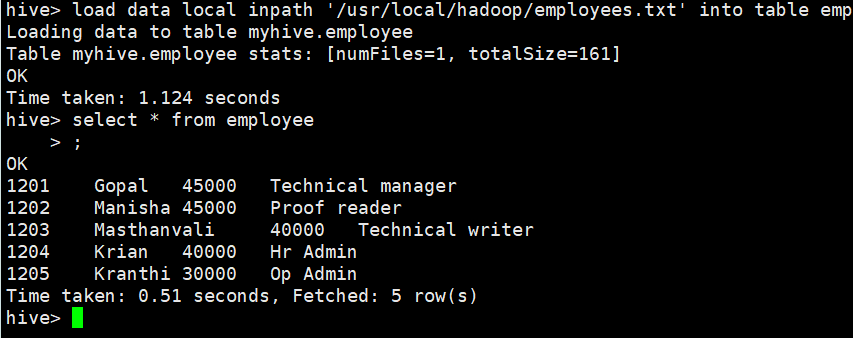
\includegraphics[scale=1.0]{figures/17.png}
\caption{结果}\label{fig:label2}
\end{figure}

(2)在分布式目录中查看hive内表信息,先查看地址,然后再查看信息

\begin{lstlisting}[language={[ANSI]C}]
hadoop fs -lsr /user/
hadoop fs -text /user/hive/warehouse/myhive.db/employee/employees.txt
\end{lstlisting}

\begin{figure}[ht]
\centering
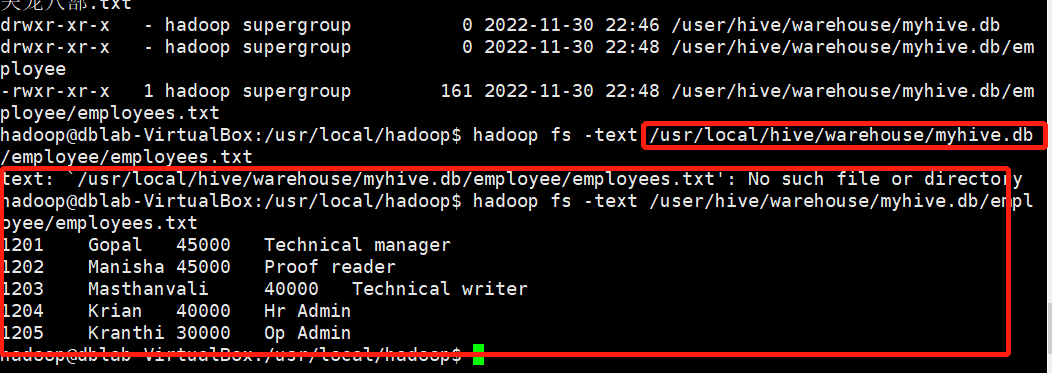
\includegraphics[scale=0.8]{figures/18.png}
\caption{数据查看}\label{fig:label2}
\end{figure}

\newpage
(3)在hive中查看本地数据

\begin{lstlisting}[language={[ANSI]C}]
!ls /usr/local/hadoop
\end{lstlisting}

\begin{figure}[ht]
\centering
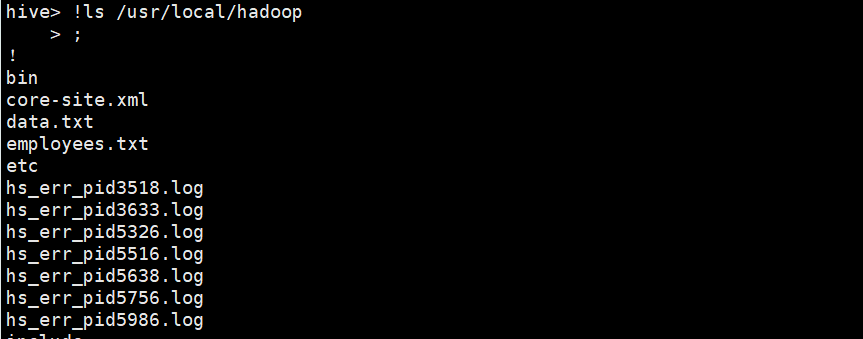
\includegraphics[scale=1.0]{figures/19.png}
\caption{本地数据查看}\label{fig:label2}
\end{figure}

(4)在hive中执行hdfs
\begin{lstlisting}[language={[ANSI]C}]
dfs -ls /;
\end{lstlisting}

\begin{figure}[ht]
\centering
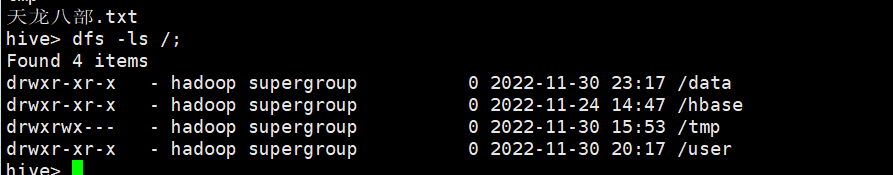
\includegraphics[scale=1.0]{figures/20.png}
\caption{本地数据查看}\label{fig:label2}
\end{figure}

\section{Sqoop}

\subsection{安装sqoop和问题处理}

(1)在官网下载mysql包和sqoop包
\begin{lstlisting}[language={[ANSI]C}]
#解压到本地
tar -zxvf sqoop-1.4.7.bin__hadoop-2.6.0.tar.gz -C /usr/local/
cd /usr/local/
#改名字
sudo mv  sqoop-1.4.7.bin__hadoop-2.6.0 sqoop
cd /usr/local/sqoop/conf
mv sqoop-env-template.sh sqoop-env.sh
\end{lstlisting}

(2)修改环境变量
\begin{lstlisting}[language={[ANSI]C}]
sudo vim sqoop-env.sh
export HADOOP_COMMON_HOME=/usr/local/hadoop
export HADOOP_MAPRED_HOME=/usr/local/hadoop
export HIVE_HOME=/usr/local/hive
\end{lstlisting}

\begin{figure}[ht]
\centering
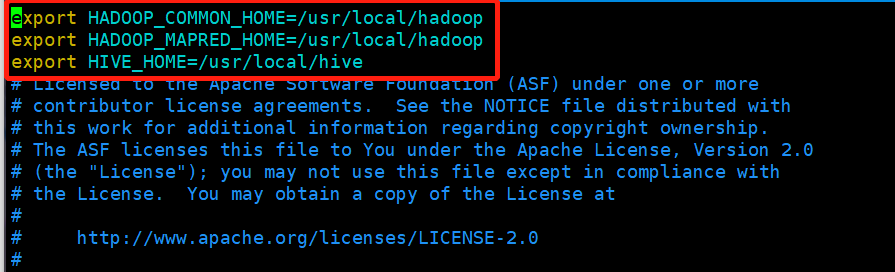
\includegraphics[scale=1.0]{figures/22.png}
\caption{环境变量}\label{fig:label2}
\end{figure}

(3)将mysql的驱动包mysql-connector-java-5.1.46-bin.jar复制到Sqoop安装目录下的lib 文件夹中

\begin{lstlisting}[language={[ANSI]C}]
sudo vim ~/.bashrc

#sqoop,下面的是放进去的环境变量
export SQOOP_HOME=/usr/local/sqoop-1.4.7.bin__hadoop-2.6.0
export PATH=$PATH:$SQOOP_HOME/bin
source ~/.bashrc
\end{lstlisting}

\begin{figure}[ht]
\centering
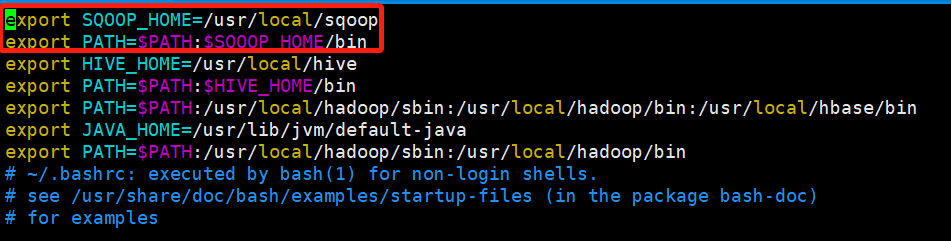
\includegraphics[scale=0.9]{figures/23.png}
\caption{环境变量}\label{fig:label2}
\end{figure}

\newpage
(4)最后查看版本

\begin{lstlisting}[language={[ANSI]C}]
cd /usr/local/sqoop
sqoop version
\end{lstlisting}


\begin{figure}[ht]
\centering
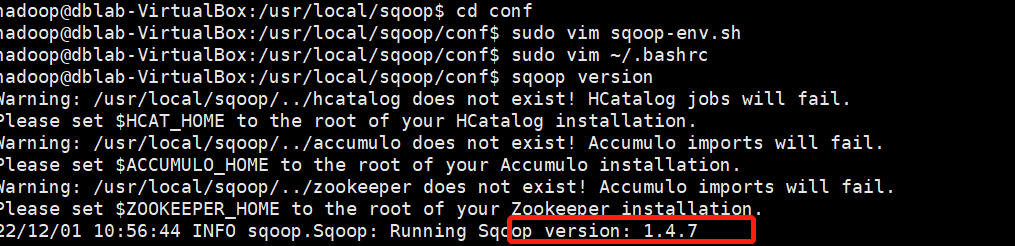
\includegraphics[scale=0.8]{figures/24.png}
\caption{sqoop版本}\label{fig:label2}
\end{figure}

(5)为了处理sqoop连接mysql时需要用户密码,特此查看与改密码;

\begin{lstlisting}[language={[ANSI]C}]
mysql -u root -p
#此时我是没有密码登录的
show databases;
use mysql;
show tables;
select user,host,authentication_string from user;
update user set authentication_string='密码' where user='root';
#最后刷新权限
flush privileges;
\end{lstlisting}

\begin{figure}[ht]
\centering
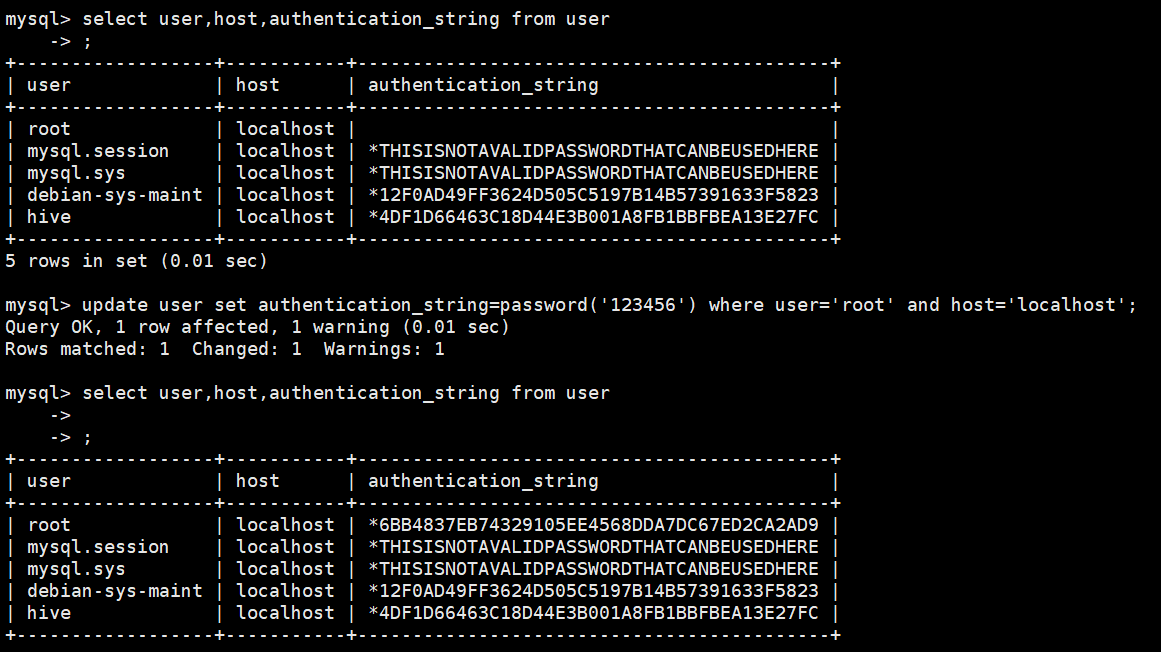
\includegraphics[scale=0.7]{figures/111.png}
\caption{修改mysql密码}\label{fig:label2}
\end{figure}


\newpage
\subsection{sqoop基本基本操作}
(1)基本操作
\begin{lstlisting}
#检查是否连接数据库
#查看数据库列表
cd /usr/local/sqoop
bin/sqoop list-databases --connect jdbc:mysql://localhost:3306/ --username xxxx --password xxxxxx
#查看命令
sqoop help
\end{lstlisting}

(2)关于sqoop与mysql互连时的版本不匹配问题

\begin{figure}[ht]
\centering
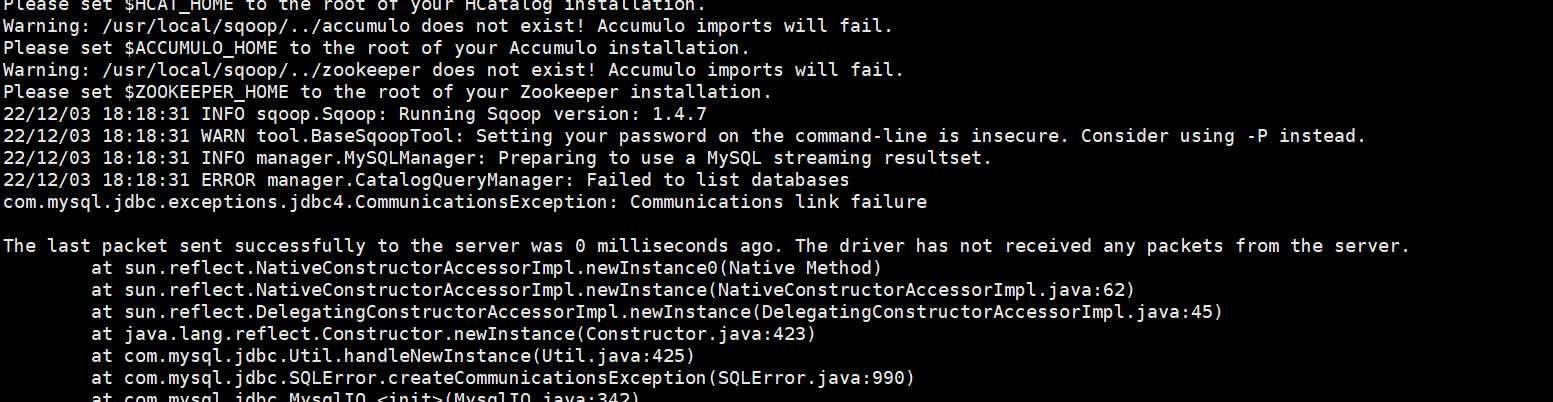
\includegraphics[scale=0.6]{figures/222.png}
\caption{报错信息}\label{fig:label2}
\end{figure}

\newpage
(3)重新下载包,下载相对应的jdbc驱动程序

\begin{figure}[ht]
\centering
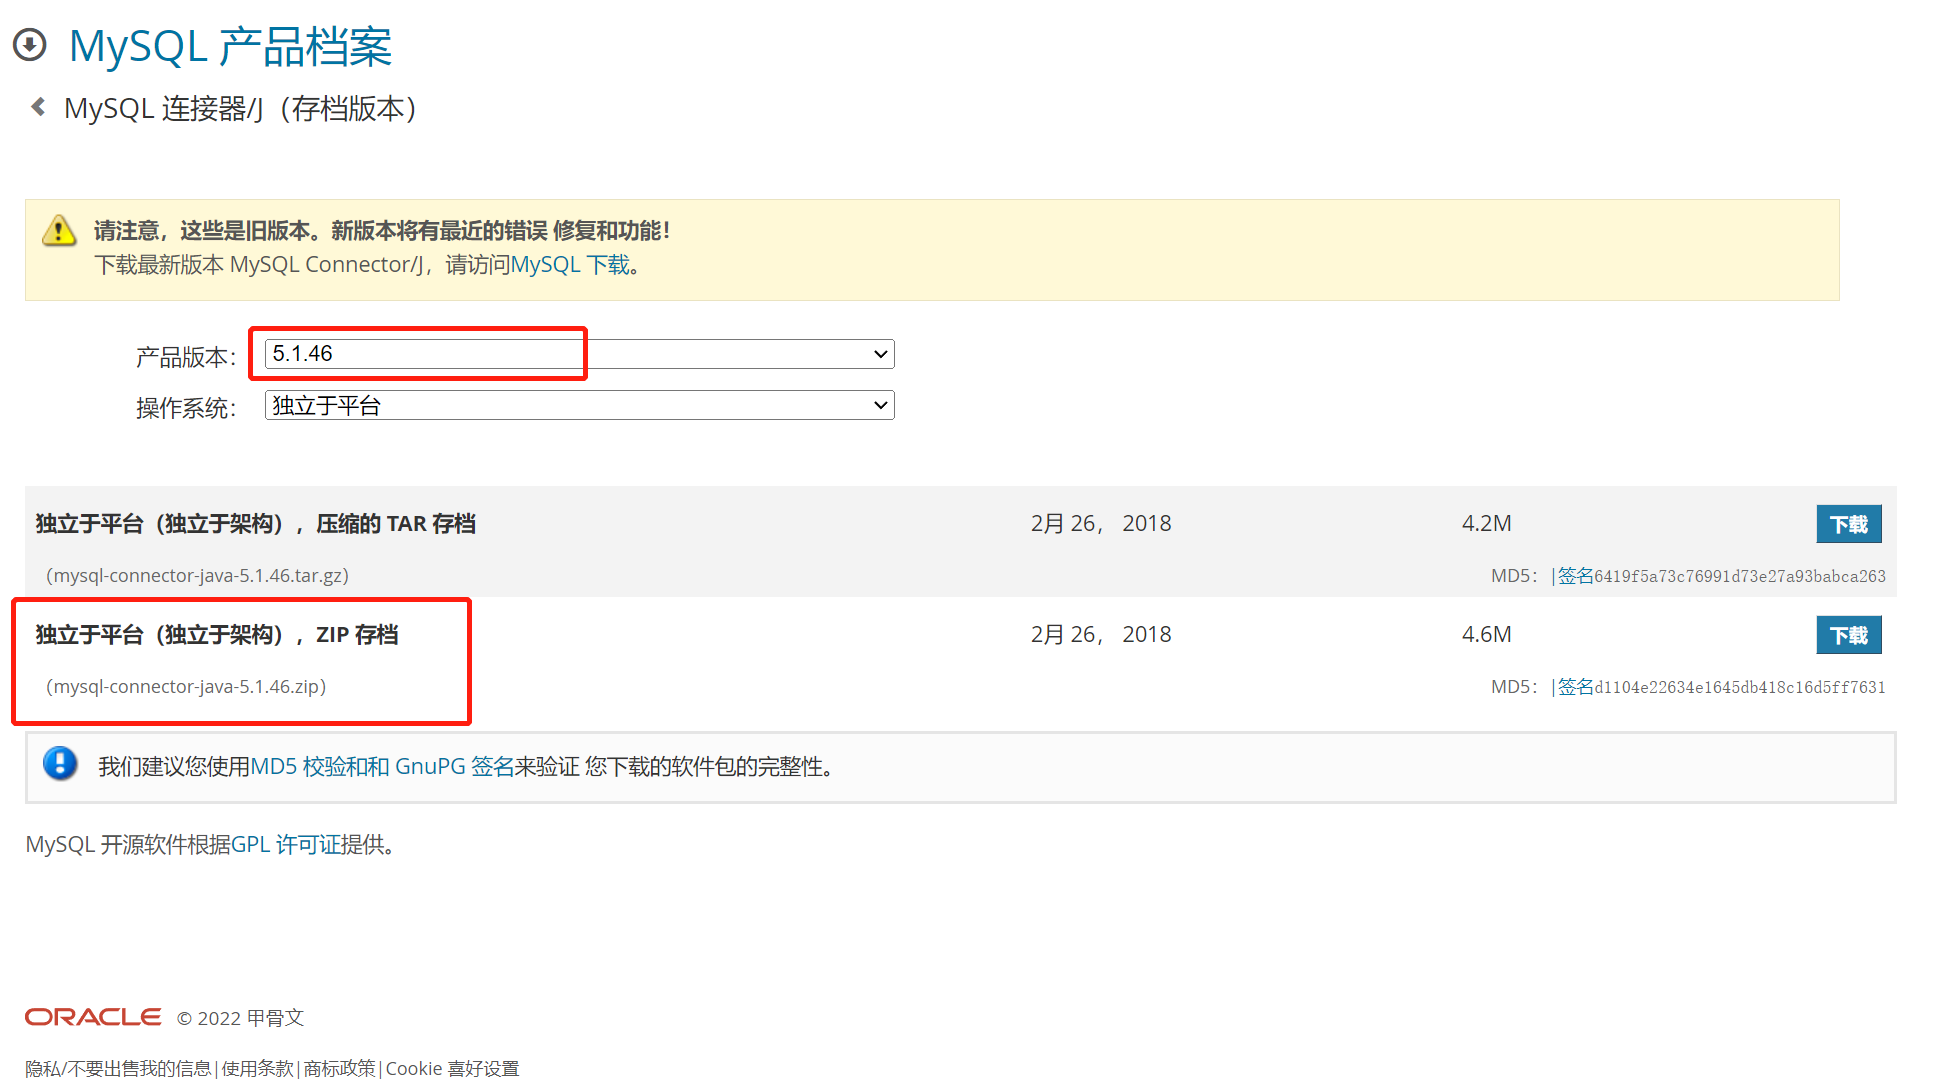
\includegraphics[scale=0.4]{figures/555.png}
\caption{报错信息}\label{fig:label2}
\end{figure}

(4)把解压好的包,放在sqoop中

\begin{lstlisting}
cd
ls
pwd
sudo cp /home/hadoop/mysql-connect-5.1.46.bin.jar /usr/local/sqoop/lib
\end{lstlisting}

\subsection{sqoop实操}
(1)关于sqoop与mysql成功,显示数据库

\begin{lstlisting}
bin/sqoop list-databases --connect jdbc:mysql://localhost:3306/ --username xxxx --password xxxxxx
\end{lstlisting}

\begin{figure}[ht]
\centering
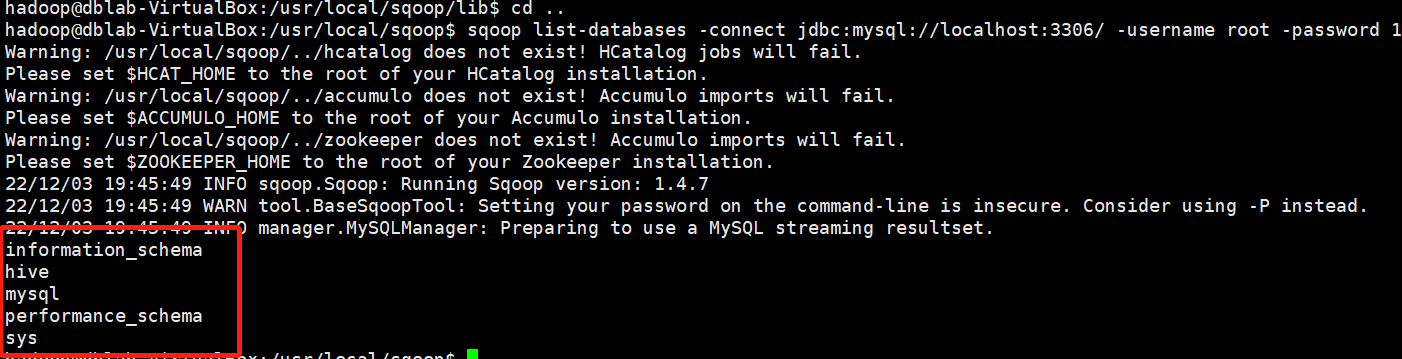
\includegraphics[scale=0.6]{figures/333.png}
\caption{成功连接数据库}\label{fig:label2}
\end{figure}

\newpage
(2)查看表

\begin{lstlisting}
sqoop list-tables -connect jdbc:mysql://localhost:3306/hive -username root -password 123456
\end{lstlisting}

\begin{figure}[ht]
\centering
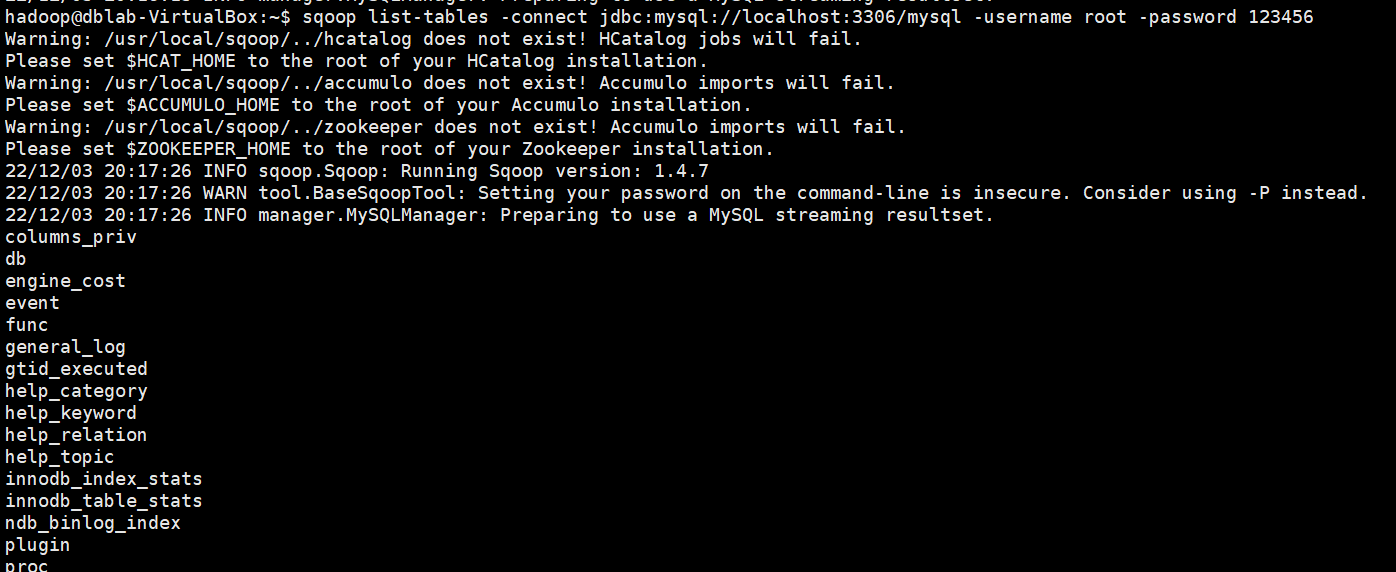
\includegraphics[scale=0.6]{figures/444.png}
\caption{查看数据表}\label{fig:label2}
\end{figure}

(3)为了让sqoop与hive互通,要配置文件

\begin{lstlisting}[language={[ANSI]C}]
#此安装包为自己安装的版本
cp /home/hive/lib/hive-common-1.2.1.jar /home/sqoop/lib/
\end{lstlisting}


\section{基于mysql,hive,sqoop的案例}

\subsection{实例}
(1)先进去mysql,创建数据库,数据表,内容。

\begin{lstlisting}[language={[ANSI]C}]
mysql -u root -p
create database sample;
use sample;
create table student(number char(9) primary key, name varchar(10));
insert into student values('01','zhangsan');
insert into student values('02','lisi');
insert into student values('03','wangwu');
\end{lstlisting}

\begin{figure}[ht]
\centering
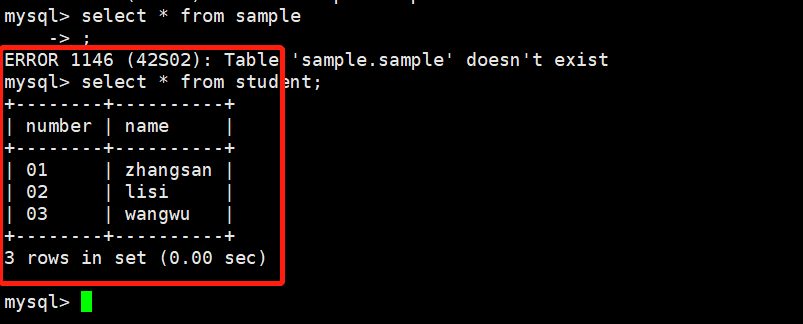
\includegraphics[scale=1.0]{figures/25.png}
\caption{创建的数据表}\label{fig:label2}
\end{figure}

\newpage
(2)进入hive,然后创建相同的数据库和数据表,还要表的字段名
\begin{lstlisting}[language={[ANSI]C}]
cd /usr/local/hive
hive
create database sample;
use sample;
create table student(number STRING, name STRING) row format delimited fields terminated by ',';
\end{lstlisting}

(3)通过sqoop把数据库的内容放到hive里面

\begin{lstlisting}
sqoop import --connect jdbc:mysql://localhost:3306/sample --username root --password 123456 --table student --fields-terminated-by ',' --delete-target-dir --num-mappers 1 --hive-import --hive-database sample --hive-table student
\end{lstlisting}

(4)查看hive,看是否传输进去

\begin{lstlisting}[language={[ANSI]C}]
cd /usr/local/hive
hive
use sample;
select * from student;
\end{lstlisting}

\begin{figure}[ht]
\centering
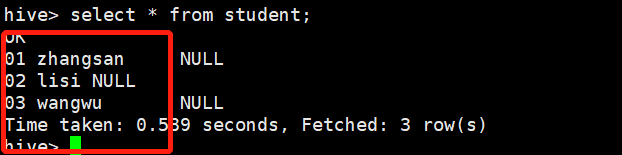
\includegraphics[scale=1.3]{figures/26.png}
\caption{传输成功}\label{fig:label2}
\end{figure}

(5)上面的是通过mysql传输到hive,现在是hive传输到mysql,只用把import转export
\begin{lstlisting}[language={[ANSI]C}]
sqoop export --connect jdbc:mysql://localhost:3306/sample
->--username root
->--password 123456
->--table student
->--fields-terminated-by ','
-> --delete-target-dir
->--num-mappers 1
->--hive-export
->--hive-database sample
->--hive-table student
\end{lstlisting}

\subsection{总结}

(1)sqoop列出 MySQL 数据库中的所有数据库
\begin{lstlisting}
sqoop list-databases -connect jdbc:mysql://localhost:3306/ -username root -password 123456
\end{lstlisting}

(2)连接MySQL并列出 sample数据库中的表
\begin{lstlisting}
sqoop list-tables -connect jdbc:mysql://localhost:3306/sample -username root -password 123456
\end{lstlisting}

(3)将关系型数据的表结构复制到hive中,只是复制表的结构,表中的内容没有复制过去。
\begin{lstlisting}
sqoop create-hive-table -connect jdbc:mysql://localhost:3306/sample -table student -username root -password 123456 -hive-table test
\end{lstlisting}

(4)从关系数据库导入文件到Hive中。
\begin{lstlisting}
sqoop import --connect jdbc:mysql://localhost:3306/sample --username root --password 123456 --table student --delete-target-dir --num-mappers 1 --hive-import --hive-database default --hive-table test
\end{lstlisting}

(5)从数据库导出表的数据到 HDFS 上文件。
\begin{lstlisting}
sqoop import -connect jdbc:mysql://localhost:3306/sample -username root -password 123456 -table student --num-mappers 1 -targetdir /user/test
\end{lstlisting}

(6)从数据库增量导入表数据到 HDFS中。
\begin{lstlisting}
sqoop import -connect jdbc:mysql://localhost:3306/sample -username root -password 123456 -table student --num-mappers 1 -targetdir /user/test -check-column number -incremental append -last-value 0
\end{lstlisting}

\section{关于磁盘不够的问题解决}

(1)查询磁盘是否有空间,如果没看足够的磁盘,就要在windows下,给予某个已经固定的虚拟机内存。

\begin{lstlisting}
df -hl
\end{lstlisting}

\begin{figure}[ht]
\centering
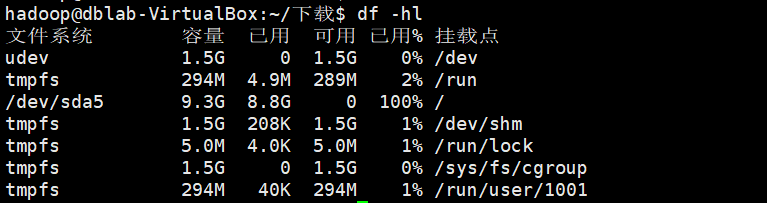
\includegraphics[scale=1.2]{figures/27.png}
\caption{查看空间}\label{fig:label2}
\end{figure}

(2)查看磁盘信息,这里我们重点关注/dev/sda3的system这个属性,表示是Linux默认的磁盘管理机制。

\begin{lstlisting}
fdisk -l
\end{lstlisting}

\begin{figure}[ht]
\centering
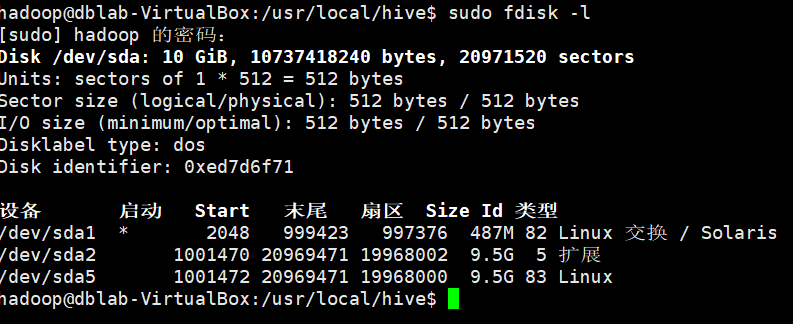
\includegraphics[scale=0.9]{figures/28.png}
\caption{查看磁盘信息}\label{fig:label2}
\end{figure}

Linux默认的磁盘管理机制这种没办法直接动态扩容,除非杀死/dev/sda5这个分区的挂载点也就是根目录里面运行的进程。

(3)在设置里面扩容磁盘,然后对磁盘进行分区,但是可能会把文件损坏。
\begin{lstlisting}
fdisk /dev/sdb
\end{lstlisting}

(4)直接格式化磁盘,也建议不要做,建议如果想安装全部软件,在开始时就直接调到30g以上。
\begin{lstlisting}
mkfs.ext4 /dev/sdb
\end{lstlisting}

(5)总结:磁盘扩容尝试了直接在windows系统操作,但是容易把虚拟机搞坏。建议扩容后分区,比较靠谱,也比较简单。


%%%%%%%%%%%%%%%%%%%%报告中涉及的安装包版本和地址%%%%%%%%%%%%%%%%%%%%%%%%%%%%%%%%%%%%%%%%%%%%%%%%%%%%%%%%%%%%%%%%%%%%%%%%%%
\newpage

\begin{thebibliography}{99}\addcontentsline{toc}{section}{报告中涉及的安装包和地址}
\wuhao{
\bibitem{huang}sqoop-1.4.7的官方地址.https://attic.apache.org/projects/sqoop.html.

\bibitem{jiang}mysql-connector-java-5.1.40的官方地址.https://dev.mysql.com/downloads/connector/j/.

\bibitem{jiang}apache-hive-1.2.1-bin的官方地址.https://dblab.xmu.edu.cn/blog/1591/.


}
\end{thebibliography}


\end{document}
